\chapter{Ancora sull'AI}

\section{AI or not AI This is the Dilemma}

\subsection{Il Watermark}

\dfn{Watermark}{
  Il watermark consiste in cambiamenti non visibili in alcuni pixel chiavi che possono essere individuati dalla macchina.
}

\begin{figure}[H]
    \centering
    
\includegraphics[scale=0.5]{02E/wm.png}
    \caption{Immagine con watermark.}
\end{figure}

\nt{Uno dei provvedimenti dell'amministrazione Biden per "difendersi" da watermark è stato quello di dire: inseriamo del watermark che indichi se un'immagine è AI-generated.}

\qs{}{Questa è una soluzione ragionevole?}

\begin{itemize}
  \item Se è possibile introdurlo allora esisterà un AI in grado di rimuoverlo. 
  \item Questa proposta garantisce Microsoft, openAI, Google che se ne lavano le mani. Però le aziende non americane non hanno alcun obbligo di applicare il watermark.
  \item Inoltre il fatto che una foto abbia il watermark, in un'epoca di cospirazionismo, non significa nulla\footnote{God, how much I hate humanity.}.
\end{itemize}

\subsection{Il Copyright}

Tutti i vari modelli di AI generativa sono stati addestrati su tutti i dati del mondo, principalmente il web (anche su materiale soggetto a copyright). Per esempio alcuni siti come z-library o il web archive\footnote{Entrambi consigliatissimi, da visitare almeno una volta nella vita, sono la nuova biblioteca di Alessandria.} in cui sono presenti contenuti piratati. I vari LLM hanno probabilmente assorbito anche quei contenuti. Ovviamente quella merda che è Google ha detto: eh, ma se è lì sul web allora lo posso prendere, se non lo volevano non lo dovevano pubblicare (a parte che è l'esatto opposto del meccanismo di copyright, ma forse non si rendono conto che è la stessa argomentazione che utilizzano gli stupratori nei confronti della loro vittima). Oppure openAI che chiede alle persone di indicare quali pagine non vogliono sia preso dal crawler. Tuttavia questo non funziona, per esempio con i siti di mirroring.

\begin{figure}[H]
    \centering
    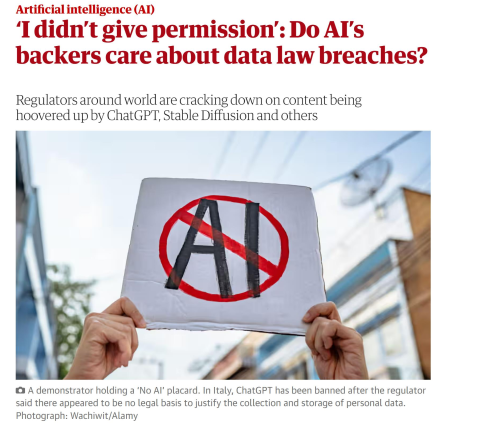
\includegraphics[scale=0.65]{02E/ai.png}
    \caption{Protestante con cartello.}
\end{figure}






